\begin{exercise}
Geben Sie alle Lösungen des folgenden Systems an:
\begin{align*}
  y^{\prime}(t) = \begin{pmatrix}
    3t -1 & 1 - t \\ t + 2 & t - 2
  \end{pmatrix}
  y(t) +
  \begin{pmatrix}
    t\exp(t^2) \\ \exp(t^2))
  \end{pmatrix}
\end{align*}
\end{exercise}
\begin{solution}
Wir kennen aus Aufgabe 4.3 die Fundamentalmatrix des entsprechenden homogenen Systems mit
\begin{align*}
Y(t) = \begin{pmatrix*}[c]
  \exp(t^2) & \exp(t^2-3t)(\frac{1}{3}t - \frac{2}{9}) \\
  \exp(t^2) & \exp(t^2-3t)(\frac{1}{3}t + \frac{7}{9})
\end{pmatrix*}.
\end{align*}
Nun können wir Satz 3.17 welcher uns durch Variation der Konstanten folgende
Lösungsformel für beliebige inhomogene Systeme liefert:
\begin{align*}
  y(t) = Y(t)(Y(t_0))^{-1}y_0 + Y(t)\int_{t_0}^{t}(Y(s))^{-1}b(s)ds
\end{align*}
Wir berechnen zuerst
\begin{align*}
  \tilde{y}(t) :&= \int_{t_0}^{t}(Y(s))^{-1}b(s)ds = \\
  &=
  \int_{t_0}^{t}  \begin{pmatrix*}[c]
      \exp(s^2) & \exp(s^2-3s)(\frac{1}{3}s - \frac{2}{9}) \\
      \exp(s^2) & \exp(s^2-3s)(\frac{1}{3}s + \frac{7}{9})
    \end{pmatrix*}^{-1}
    \begin{pmatrix}
      t\exp(t^2) \\ \exp(t^2)
    \end{pmatrix}ds \\
    & = \int_{t_0}^{t}  \begin{pmatrix*}[c]
      \frac{3s^2 + 4s + 2}{9} \\
      \exp(3s)(1 - s)
    \end{pmatrix*}ds = \begin{pmatrix*}[c]
      \frac{(t-t_0)^3 + 2(t-t_0)^2 + 2(t-t_0)}{9} \\
      \frac{\exp(3t)(4 - 3t) + \exp(3t_0)(3t_0 - 4)}{9}
    \end{pmatrix*}
\end{align*}
für $t_0 = 0$ also
\begin{align*}
  \tilde{y}(t) = \begin{pmatrix*}[c]
    \frac{t^3 + 2t^2 + 2t}{9} \\
    \frac{\exp(3t)(4 - 3t) - 4}{9}
  \end{pmatrix*}
\end{align*}
Jede Lösung des Systems hat also die Form $y = \underbrace{Y\cdot\tilde{y}}_{=y_p} + \hat{y}$ wobei $\hat{y}$ Lösung des homogenen Systems ist, d.h. $\hat{y}(t) = Y(t)\cdot c$ mit $c \in \R^2$. Insgesamt $ y = Y\cdot (\tilde{y} + c)$.

und verwenden das um die Lösung zu erhalten.
\begin{align*}
  y(t) &= \begin{pmatrix*}[c]
    \exp(t^2) & \exp(t^2-3t)(\frac{1}{3}t - \frac{2}{9}) \\
    \exp(t^2) & \exp(t^2-3t)(\frac{1}{3}t + \frac{7}{9})
  \end{pmatrix*}
  \begin{pmatrix*}[c]
    \exp(t_0^2) & \exp(t_0^2-3t)(\frac{1}{3}t_0 - \frac{2}{9}) \\
    \exp(t_0^2) & \exp(t_0^2-3t)(\frac{1}{3}t_0 + \frac{7}{9})
  \end{pmatrix*}
  \begin{pmatrix}
    y_0^1 \\ y_0^2
  \end{pmatrix}
  +
  \begin{pmatrix*}[c]
    \exp(t^2) & \exp(t^2-3t)(\frac{1}{3}t - \frac{2}{9}) \\
    \exp(t^2) & \exp(t^2-3t)(\frac{1}{3}t + \frac{7}{9})
  \end{pmatrix*}
  \tilde{y}(t) \\
    &=
  \begin{pmatrix*}[c]
    \exp(t^2) & \exp(t^2-3t)(\frac{1}{3}t - \frac{2}{9}) \\
    \exp(t^2) & \exp(t^2-3t)(\frac{1}{3}t + \frac{7}{9})
  \end{pmatrix*}
    \left( \begin{pmatrix*}[c]
        y_0^1\exp(t_0^2) + y_0^2\exp(t_0^2-3t)(\frac{1}{3}t_0 - \frac{2}{9}) \\
        y_0^1\exp(t_0^2) + y_0^2\exp(t_0^2-3t)(\frac{1}{3}t_0 + \frac{7}{9})
      \end{pmatrix*}
      + \tilde{y}(t) \right) \\
      &= \begin{pmatrix*}[c]
        \exp(t^2) & \exp(t^2-3t)(\frac{1}{3}t - \frac{2}{9}) \\
        \exp(t^2) & \exp(t^2-3t)(\frac{1}{3}t + \frac{7}{9})
      \end{pmatrix*}
      \left(\begin{pmatrix*}[c]
          y_0^1\exp(t_0^2) + y_0^2\exp(t_0^2-3t)(\frac{1}{3}t_0 - \frac{2}{9}) \\
          y_0^1\exp(t_0^2) + y_0^2\exp(t_0^2-3t)(\frac{1}{3}t_0 + \frac{7}{9})
        \end{pmatrix*} +
      \tilde{y}(t) \right)\\
        &= \begin{pmatrix*}[c]
          \exp(t^2) & \exp(t^2-3t)(\frac{1}{3}t - \frac{2}{9}) \\
          \exp(t^2) & \exp(t^2-3t)(\frac{1}{3}t + \frac{7}{9})
        \end{pmatrix*}
        \left(\begin{pmatrix*}[c]
            y_0^1\exp(t_0^2) + y_0^2\exp(t_0^2-3t)(\frac{1}{3}t_0 - \frac{2}{9}) \\
            y_0^1\exp(t_0^2) + y_0^2\exp(t_0^2-3t)(\frac{1}{3}t_0 + \frac{7}{9})
          \end{pmatrix*} +
        \begin{pmatrix*}[c]
            \frac{(t-t_0)^3 + 2(t-t_0)^2 + 2(t-t_0)}{9} \\
            \frac{\exp(3t)(4 - 3t) + \exp(3t_0)(3t_0 - 4)}{9}
          \end{pmatrix*} \right) =
\end{align*}
\FloatBarrier
\begin{figure}
    \centering
    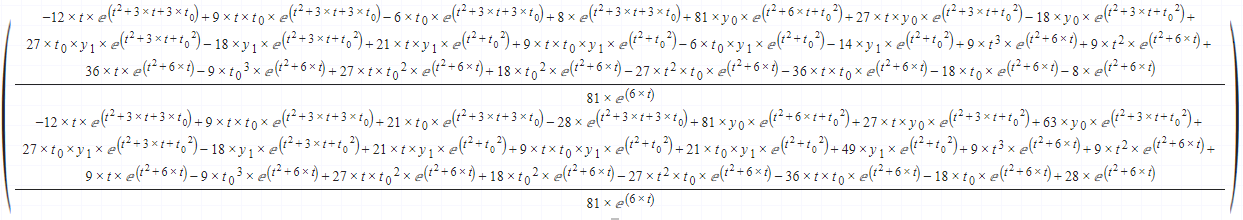
\includegraphics[width=\linewidth]{matrix.png}
\end{figure}
\FloatBarrier
\end{solution}
